\documentclass{marine_2015}
     
\usepackage{graphicx}
\usepackage{amsmath}
\usepackage{amsfonts}
\usepackage{amssymb}
\usepackage{floatrow}
\usepackage{xfrac}
\floatsetup[table]{capposition=top}

\newcommand{\Amat}{\ensuremath{\mathbb{A}}}
\newcommand{\Bmat}{\ensuremath{\mathbb{B}}}
\newcommand{\bvec}{\ensuremath{\mathbf{b}}}
\newcommand{\uvec}{\ensuremath{\mathbf{u}}}
\newcommand{\Uvec}{\ensuremath{\mathbf{U}}}
\newcommand{\Pvec}{\ensuremath{\mathbf{P}}}
\newcommand\blfootnote[1]{%
  \begingroup
  \renewcommand\thefootnote{}\footnote{#1}%
  \addtocounter{footnote}{-1}%
  \endgroup
}

\newcommand{\bend}{\ensuremath{\text{Bend}\left|\text{P}\right|\text{y}}}
\newcommand{\RM}{\ensuremath{RM}}
\newcommand{\inner}[2]{\ensuremath{\left(#1, #2\right)}}
\newcommand{\rinner}[2]{\ensuremath{\left(#1, #2\right)_r}}
\newcommand{\tuple}[2]{\ensuremath{\left[#1, #2\right]}}

\newcommand{\ainner}[2]{\ensuremath{a\left(#1, #2\right)}}
\newcommand{\arinner}[2]{\ensuremath{a_r\left(#1, #2\right)}}
\newcommand{\binner}[2]{\ensuremath{b\left(#1, #2\right)}}
\newcommand{\brinner}[2]{\ensuremath{b_r\left(#1, #2\right)}}

\newcommand{\Linner}[1]{\ensuremath{L\left(#1\right)}}
\newcommand{\Vh}{\ensuremath{V_{\mathbf{n}}}}
\newcommand{\Qh}{\ensuremath{Q_{\mathbf{m}}}}

\newcommand{\norm}[1]{\ensuremath{\left\|#1\right\|}}
\newcommand{\vvec}[1]{\ensuremath{\pmb{#1}}}
\newcommand{\deriv}[2]{\ensuremath{\frac{\mathrm{d}#1}{\mathrm{d}#2}}}
\newcommand{\tderiv}[2]{\ensuremath{\tfrac{\mathrm{d}#1}{\mathrm{d}#2}}}

\bibliographystyle{plain}

\title{
  BEND$\left|\text{P}\right|$Y: PYTHON FRAMEWORK FOR COMPUTING BENDING OF COMPLEX PLATE-BEAM SYSTEMS
}

\author{MIKAEL MORTENSEN$^{1, 2}$ AND MIROSLAV KUCHTA$^{1}$ AND KENT-ANDRE MARDAL$^{1, 2}$ 
  \blfootnote{
    Acknowledgements: K. A. Mardal and M. Mortensen acknowledge support through a 
    Center of Excellence grant from the Research Council of Norway to the Center 
    for Biomedical Computing at Simula Research Laboratory. The work of K. A. 
    Mardal was also supported by the Research Council of Norway through grant no. 209951.
  }
}

\heading{Mikael Mortensen, Miroslav Kuchta and Kent-Andre Mardal}

\address{$^{1}$
Department of Mathematics, Division of Mechanics, University of Oslo,\\
0316 Oslo, Norway
  \and
$^{2}$ 
Center for Biomedical Computing, Simula Research Laboratory,\\
P.O. Box 134, No-134 Lysaker, Norway
}

\keywords{biharmonic equation, Lagrange multipliers, Schur complement}

\abstract{
We present a light-weight Python module for computing small deformations of a 
single plate supported by an arbitrary number of possibly intersecting
stiffeners. We show how the problem fits into the framework of abstract 
saddle point problems and how this abstraction can be exploited for clean design 
of the code. Stability properties of the resulting linear systems for two different 
sets of basis functions, namely, the eigenfunctions of the biharmonic operator 
and specialized Legendre polynomials are discussed. 
}

\begin{document}

\section{Introduction}
% What are we solving?
In this paper we discuss Galerkin methods for finding the equilibrium state of a 
physical system formed by a loaded thin plate and several beams which are constrained 
to deform together with the plate. Let us denote as $\Omega$ the subset of the
Euclidean plane occupied by the plate. We shall consider the plate supported by
$k$ beams labeled by index $r$ from the index set $R=\left\{1, 2, \cdots, k\right\}$. 
Further, each beam is a curve $\Gamma_r=\left\{x\in\Omega, x=F_r\left(s\right),
s\in\left[s_0, s_1\right]=\mathcal{I}\right\}$ that is described by an invertible mapping
$F_r:\mathcal{I}\mapsto \Omega$ with Jacobian $J_r$. Note that for straight beams, 
which are the main focus of the present work, the Jacobian is simply the length of 
the beam divided by the length of the interval. In addition we shall for
simplicity require that the mapping $F_r$ satisfies two additional constraints 
$F_r\left(s_0\right), F_r\left(s_1\right)\in\partial\Omega$. The endpoints of
the beam are thus required to lie on the boundary of the plate $\partial\Omega$.
Equivalently, the additional constraints ensure that no beam ends inside the plate.
The equilibrium state of the physical system formed by the plate supported with 
the beams is found as the solution of a constrained minimization problem
\begin{equation}
  \label{eq:foo}
  u = \min_{v\in V} \mathcal{E}\left(v\right)\quad\text{ and }\quad u_0\circ F_r
  = u_r, r=1, 2, \cdots k,
\end{equation}
where the energy functional $\mathcal{E}:V\mapsto\mathbb{R}$ is defined as
\[
  \mathcal{E}\left(u\right)=
    \frac{E_0}{2}\displaystyle\int_{\Omega}\Delta u_0\,\Delta u_0+
    \sum_{r=1}^k\frac{E_r}{2}\int_{\mathcal{I}}
  \deriv{^2u_r}{s^2}\deriv{^2u_r}{s^2}J_r^{-3}
  -\displaystyle\int_{\Omega}f u_0.
\]
Here $V=V_0\times V_1 \times\cdots\times V_k$ is a function space with $k+1$
components. The first component $V_0$ contains functions that map the plate
domain $\Omega$ to real numbers and is therefore the space where the plate's
vertical displacement $u_0$ is found. The remaining components in $V$ contain the 
vertical displacements of individual beams $u_r$, i.e., the scalar 
functions whose domain is the interval $\mathcal{I}$. The system is loaded by
the load $f$ while $E_0, E_r, r\in R$ are constant parameters that, 
following the Kirchhoff-Love and Euler-Bernoulli hypothesis (see, e.g., \cite{reddy}), 
depend on the material and the geometry.

Introducing $k$ Lagrange multipliers $\lambda_k\in Q_k$, where the functions in 
$Q_k$ map the interval $\mathcal{I}$ to scalars, the constrained problem 
(\ref{eq:foo}) can be equivalently written as a search for extrema of the Lagrangian
$\mathcal{L}:V\times Q\mapsto \mathbb{R}$,
\begin{equation}
  \label{eq:bar}
\mathcal{L}\left(u, \lambda\right) = \mathcal{E}\left(u\right) +
  \sum_{r=1}^k\int_{\mathcal{I}}\left(u_0\circ F_r - u_r\right)\lambda_r J_r.
\end{equation}
The space $Q=Q_1\times Q_2\times\cdots\times Q_k$ has $k$ components with $r$-th
component containing a Lagrange multiplier that enforces the matching deformation 
constraint on the beam with index $r$. We note that the unconstrained problem (\ref{eq:bar}) 
is solvable only for suitable pair of spaces $V, Q$ for which the requirements of the
Babu\v{s}ka-Brezzi \cite{babuska, brezzi} theory are satisfied.

% It can be solved with FEM but simple geometry ... global functions, spectral
% Galerkin
For plate $\Omega$ with complex shape the finite element method is arguably 
the most suitable method to solve the problem (\ref{eq:bar}). If, on the other hand, the
domain is simple (e.g. separable), the Galerkin method with globally supported basis functions
that take advantage of the structure of the domain (and the underlying PDE) can 
be applied. Note that the finite element method is an instance of the Galerkin 
method with trial/test\footnote{We consider Bubnov-Galerkin method where the
trial and test spaces are equal.} spaces spanned by the functions with local support. 
Regardless of the basis functions employed, the stable discretization of problem (\ref{eq:bar})
requires that the Babu\v{s}ka-Brezzi conditions be satisfied on the constructed
finite dimensional spaces. We remark that in addition to stability
considerations the finite element discretization of the problem is also complicated
by the presence of the biharmonic operator, which requires techniques for fourth order 
problems (see, e.g., \cite{brenner}). The approximations of $V$ must be constructed 
from $C^1$-continuous elements, e.g., the Argyris element \cite{argyris}, or non-conforming 
elements like the Morley element \cite{morley}. Alternatively, discontinuous elements with 
suitable stabilization \cite{brennerip} can be used. 

Here we shall consider the plate as a simply connected rectangular domain and as
such focus on Galerkin methods with test functions having global support.
Further, the two selected basis are designed for fourth order problems and thus 
only the Babu\v{s}ka-Brezzi theory needs to be considered to derive a stable
discretization of problem (\ref{eq:bar}). The methods are discussed within a
framework for abstract saddle point problems reviewed in Section
\ref{sec:abstract}. The framework serves to identify the few common
elements (matrices) that are required to easily introduce Galerkin discretizations of
(\ref{eq:bar}) based on any set of basis functions. Properties of the two sets of
basis functions considered in this paper are then compared in Section \ref{sec:basis}.
Finally in Section \ref{sec:lbb} the inf-sup condition for the two proposed
discretizations is discussed.

\section{Abstract framework for saddle point problems}
\label{sec:abstract}
% conditions for extrema
The necessary conditions for the extreme point of the Lagrangian $\mathcal{L}$
defined in (\ref{eq:bar}) form the saddle point system of $2k+1$ equations to be 
satisfied by the $2k+1$ unknowns $\left(u, \lambda\right)\in V\times Q$. These equations read
\begin{equation}
  \label{eq:system}
  \begin{aligned}
    E_0\displaystyle\int_{\Omega}\Delta u_0\,\Delta v_0-
    \sum_{r=1}^k\int_{\mathcal{I}}v_0\lambda_r J_r &=\displaystyle\int_{\Omega}f
    v_0\quad\forall v_0\in V_0,& \\
    E_r\displaystyle\int_{\mathcal{I}}
    \deriv{^2u_r}{s^2}\deriv{^2v_r}{s^2}J_r^{-3} +
  \int_{\mathcal{I}} v_r \lambda_r J_r &= 0\quad\forall v_r\in V_r, r\in R,&\\
  \int_{\mathcal{I}}\left(u_r-u_0\right)\mu_r J_r &= 0\quad\forall \mu_r\in Q_r,
    r\in R.&\\
  \end{aligned}
\end{equation}
System (\ref{eq:system}) fits into the abstract framework for saddle point
problems (see eq. Quarteroni \cite{quarteroni}). Within the framework, existence
and uniqueness of the solution of (\ref{eq:system}) can be discussed. Here we
shall assume that the problem is indeed well-posed and instead use the abstractions
of the framework to identify the building blocks for efficient implementation
of the Galerkin method for the system. To simplify the notation we
let $\inner{\cdot}{\cdot}$ denote the $L^2$-inner product over the plate.
Moreover for $r\in R$ the weighted $L^2$-inner product over the
interval $\mathcal{I}$ with the weight $J_r$ is denoted as $\rinner{\cdot}{\cdot}$.

The abstract saddle point problem is defined in terms of bilinear forms $a:V\times V\mapsto \mathbb{R}$,
$b:Q\times V\mapsto \mathbb{R}$ and a linear form $L:V\mapsto R$. To identify these 
forms in the plate-beam system (\ref{eq:system}), let $a_0:V_0\times V_0\mapsto
\mathbb{R}$ with $\ainner{u_0}{v_0}=E_0\inner{\Delta u_0}{\Delta v_0}$ and
$a_r:V_r\times V_r\mapsto \mathbb{R}$ such that $\arinner{u_r}{v_r}=E_r\rinner{J_r^{-2}\tderiv{^2 u_r}{s^2}}{J_r^{-2}\tderiv{^2
v_r}{s^2}}$ for $r\in R$. Moreover we define $r$ bilinear forms
$b_r:Q_r\times V\mapsto\mathbb{R}$ by
$\brinner{\lambda_r}{u}=\rinner{u_0\circ F_r-u_r}{\lambda_r}$. It then follows 
that the bilinear forms $a$ and $b$ are simply
\[
  \ainner{u}{v} = \displaystyle\sum_{r=0}^{k}\arinner{u_r}{v_r}\quad\text{ and
  }\quad\binner{\lambda}{u} = \displaystyle\sum_{r=1}^{k}\brinner{\lambda_r}{u}.
\]
Finally with the linear form $\Linner{u}=\inner{f}{u_0}$ the problem
(\ref{eq:system}) is rewritten as an abstract saddle point problem: Find
$\left(u, \lambda\right)\in V\times Q$ such that
\[
%\begin{equation}
  %\label{eq:abstract_saddle}
  \ainner{u}{v} + \binner{\lambda}{v} + \binner{\mu}{u} = \Linner{v}\quad\forall
  \left(v, \mu\right)\in V\times Q.
%\end{equation}
\]

To apply the Galerkin method to system (\ref{eq:system}) we construct finite dimensional
subspaces $\Vh\subset V$ and $\Qh\subset Q$ that approximate $V$ and $Q$
respectively. As such the spaces $\Vh, \Qh$ have respectively $k+1$ and $k$
components with their individual dimensions
$\text{dim}\left(\Vh^r\right)=\mathbf{n}_r$, $\text{dim}\left(\Qh^r\right)=\mathbf{m}_r$ 
encoded in multi-indices\footnote{A multi-index $\mathbf{\iota}$ of length $n$
is an $n$-tuple of positive numbers. The size of multi-index is defined as the
sum of its components $\mathbf{\iota}_i, i=1, 2, \cdots, n$.} $\mathbf{n}\in\mathbb{R}^{k+1}, \mathbf{m}\in\mathbb{R}^k$.
From this definition it follows that $n=\text{dim}\left(\Vh\right)$ and $m=\text{dim}\left(\Qh\right)$
are the sizes of the respected multi-indices. Considering the saddle point
problem (\ref{eq:system}) on the constructed subspaces yields a symmetric
indefinite linear system
\begin{equation}
  \label{eq:sysAB}
    \begin{bmatrix}
      \mathbb{A} & \mathbb{B} \\
      \mathbb{B}^{\text{T}} & 0
    \end{bmatrix}
    \,
    \begin{bmatrix}
      \mathbf{U} \\
      \mathbf{P}
    \end{bmatrix}
    =
    \begin{bmatrix}
      \mathbf{b}\\
      0
    \end{bmatrix},
\end{equation}
for the unknown expansion coefficients $\Uvec\in\mathbb{R}^n,
\Pvec\in\mathbb{R}^m$ of the approximate solution
$\left(u_\mathbf{n}, \lambda_{\mathbf{m}}\right)\in \Vh \times \Qh$ of
(\ref{eq:system}).

Matrices $\Amat\in\mathbb{R}^{n\times n}$, $\Bmat\in\mathbb{R}^{n\times m}$ in
(\ref{eq:sysAB}) inherit the structure of the bilinear forms $a, b$. Specifically, 
the structure of $a$ translates into a block diagonal matrix $\Amat$ consisting of
$k+1$ blocks
\[
    \mathbb{A}=
    \begin{bmatrix}
      \mathbb{A}^0  &   &  &\\
                    & \mathbb{A}^1 &  &\\
                    &   &   \ddots    & \\
                    &   &   & \mathbb{A}^k\\
    \end{bmatrix},
\]
where the submatrices $\mathbb{A}^r$ are defined as $\mathbb{A}^r_{i,
j}=\arinner{\phi^r_i}{\phi^r_j}$ for $\phi^r_i, i=1, 2, \cdots \mathbf{n}_r$ the
basis functions of the component $\Vh^r$. Moreover, due to structure of $b$ the 
matrix $\Bmat$ consists of $k$ columns with block structure
\[
    \mathbb{B}=
    \begin{bmatrix}
      \mathbb{C}^1 & \mathbb{C}^2 & \cdots & \cdots & \mathbb{C}^k\\
      \mathbb{M}^1   &        0       & \cdots & \cdots &        0      \\
           0         & \mathbb{M}^2   &    0   & \cdots &   \vdots      \\
         \vdots      &       0        & \ddots & \ddots &   \vdots      \\
         \vdots      &     \vdots      & \ddots & \ddots &       0      \\
      0         &  \cdots        & \cdots & 0      &   \mathbb{M}^k     \\
    \end{bmatrix}.
\]
Each column features two sub-matrices
$\mathbb{C}^r\in\mathbb{R}^{n\times\mathbf{m}_r}$ and
$\mathbb{M}^r\in\mathbb{R}^{\mathbf{n}_r\times\mathbf{m}_r}$, which enforce the
constraint of equal deformation of the plate and $r$-th beam. The matrix
$\mathbb{C}^r$ with entries $\mathbb{C}^r_{i, j} = \rinner{\phi^0_i\circ F_r}{\psi^r_j}$ 
enforces the constraint on the plate, while matrix $\mathbb{M}^r$ defined by
$\mathbb{M}^r_{i, j}=-\rinner{\phi^r_i}{\psi^r_j}$ then enforces the constraint
on the beam. Note that the $\psi^r_j, j=1, 2,\cdots,\mathbf{m}_r$ denote the basis
functions of the Lagrange multiplier space $\Qh^r$.

It is clear from the structure of the matrices of the linear system
(\ref{eq:sysAB}) that its assembly requires three types of procedures: (i) For 
every subspace $\Vh^r$ a matrix resulting from discretization of the biharmonic operator is needed.
Note that for all the components but $\Vh^0$ the biharmonic operator is one-dimensional. 
(ii) For every pair of spaces $\Vh^r, \Qh^r, r\in R$ a negative mass
matrix $\mathbb{M}^r$ between the two spaces must be computed. (iii) Finally, for
every space $\Qh^r$ there must be a procedure for computing matrix $\mathbb{C}^r$,
which can be interpreted as a mass matrix between the restriction of $\Vh^0$ to
beam with label $r$ and the multiplier space $\Qh^r$. The number of procedures is 
thus significantly reduced if all the spaces involved in the discrete formulation 
are spanned by the same functions (e.g. all matrices $\mathbb{A}^r$ can then be
computed by one routine which takes the size of the required matrix $\mathbf{m}_r$ as an
argument). Moreover we shall set $\mathbf{m}_r=\mathbf{n}_r, r\in R$
and thus $\Vh^r=\Qh^r$ and all the matrices $\mathbb{M}^r$ are square. A further 
step to speed up the assembly is a choice of basis functions for which the matrices 
$\mathbb{M}^r$ and $\mathbb{A}^r$ are sparse and their nonzero values can be tabulated. With such basis functions 
computing the matrices $\mathbb{C}^r$ remains the only bottleneck of the assembly 
process. 

% Some comments on python bmat, sympy.lambdify vectorize numpy leggauss.
In $\text{Bend}\!\left|\text{P}\right|\!\text{y}$\footnote{The source code
can be obtained from https://github.com/MiroK/lega/tree/bendpy} the integration of matrices $\mathbb{C}^r$ is built on top of
{\tt{NumPy}}\cite{numpy} and {\tt{SymPy}}\cite{sympy} modules. Specifically, using
{\tt{SymPy}}'s {\tt{lambdify}} function, each integrand is turned from a symbolic 
representation to a lambda function which is vectorized for fast evaluation of 
{\tt{NumPy}} arrays which contains the points of the Gauss-Legendre quadrature. 
The remaining matrices of the linear system (\ref{eq:sysAB}) are sparse and 
efficiently stored in the compressed sparse row containers provided by {\tt{scipy.sparse}} module.
The two sets of basis functions which are currently supported by $\text{Bend}\!\left|\text{P}\right|\!\text{y}$
are discussed in the next section.

\section{Basis functions of the Galerkin method}
\label{sec:basis}
For sufficiently smooth solutions $\left(u, \lambda\right)$ of the saddle point
problem (\ref{eq:system}) the integration by parts yields that the solution $u$ also
satisfies the system of partial differential equations
\[
  \begin{aligned}
    E_0\Delta^2u_0 &= f\quad\text{ in }\Omega,\\
    E_r\deriv{^4 u_r}{s^4} &= 0\quad\text{ on }\mathcal{I}, r\in R,\\
    u_0 \circ F_r&= u_r\quad\text{ on }\mathcal{I}, r\in R,\\
  \end{aligned}
\]
subject to boundary conditions (i) $u_0=0, \partial_n u_0=0$ on $\partial\Omega $ and 
$u_r=0, \tderiv{u_r}{s}=0$ on $\partial\mathcal{I}$
or (ii) $u_0=0, \Delta u_0=0$ on $\partial\Omega$ and $u_r=0, \tderiv{^2u_r}{s^2}=0$ on
$\partial\mathcal{I}$. The first set of boundary conditions is known as clamped as
it fixes both the displacement and the rotation of the system on the boundary.
With the second pair of boundary conditions, referred to as simply supported boundary 
conditions, only the displacement is fixed. Both boundary conditions are supported 
in $\text{Bend}\!\left|\text{P}\right|\!\text{y}$. 

The clamped boundary conditions are enforced onto the solution by constructing
the test spaces of the Galerkin method from functions $S_i$ presented in Shen
\cite{shenpaper}. Functions $S_i$ defined over the interval
$\mathcal{I}=\left[-1, 1\right]$ are linear combinations of Legendre
polynomials where the coefficients of the combinations are chosen such that
$S_i=0, \tderiv{S_i}{s}=0$ in the endpoints of the domain. To span an $n$-dimensional 
space $\Vh^r, r\in R$ defined over the interval $\mathcal{I}$, the first 
$n$ functions $S_i$ are taken as the basis. For $n^2$-dimensional space $\Vh^0$ 
defined over rectangular plate $\Omega=\mathcal{I}\times\mathcal{I}$ we use as the 
basis functions products of the first $n$ functions in each Cartesian
direction. That is, the basis functions have the form $S_i\left(x\right)S_j\left(y\right)$. 
Further the choice of Shen basis functions yields matrices such that the one 
dimensional bending matrix $\mathbb{A}^r$ is the identity matrix while the mass 
matrix $\mathbb{M}^r$ is sparse and pentadiagonal. We refer the reader to the original paper \cite{shenpaper} 
for the tabulated non-zero entries of the matrix. Finally the matrix of the two-dimensional 
biharmonic operator $\mathbb{A}^0\in\mathbb{R}^{n^2\times n^2}$ is obtained
as a Kronecker product of one-dimensional mass matrix $\mathbb{M}\in\mathbb{R}^n$ and 
the stiffness matrix $\mathbb{C}\in\mathbb{R}^n$, i.e., $\mathbb{A}^0 = \mathbb{M}\otimes\mathbb{I} + 
2\mathbb{C}\otimes\mathbb{C} + \mathbb{I}\otimes\mathbb{M}$. We note that the
condition number of matrix $\mathbb{A}^0$ grows exponentially with $n$.

%sines
To enforce simply supported boundary conditions onto the approximate solutions of
(\ref{eq:system}) we consider test spaces constructed from functions 
$E_k=\left(\tfrac{2}{\pi}\right)^{1/2}\sin{kx}$,
which are eigenfunctions of the eigenvalue problem for the one-dimensional biharmonic 
operator
\[
  \begin{aligned}
  \deriv{^4 u}{s^4} = \lambda u\text{ in }\mathcal{I},\\
  u = \deriv{^2 u}{s^2} = 0\text{ on }\partial\mathcal{I},
  \end{aligned}
\]
with the interval $\mathcal{I}=\left[0, \pi\right]$. The corresponding
eigenvalues are $\lambda_k=k^4$. In complete analogy to the spaces spanned by
functions due to Shen, the basis of the $n$-dimensional space $\Vh^r, r\in R$ over
$\mathcal{I}$ is formed by the first $n$ eigenfunctions $E_k$. The basis of the
space $\Vh^0$ defined over $\Omega=\mathcal{I}\times\mathcal{I}$ are then formed
as tensor products. An attractive property of the eigenfunctions $E_k$ is the fact
that all the matrices $\mathbb{A}^0, \mathbb{A}^r$, $\mathbb{M}^r$ are diagonal. Indeed we
have $\mathbb{M}^r=\mathbb{I}$, while $\mathbb{A}^r\in\mathbb{R}^{n \times n},
r\in R$ takes the form $\mathbb{A}^r=\text{diag}\left(\lambda_k, k=1, 2, \cdots,
n\right)$. Finally the two-dimensional bending matrix takes the form
$\mathbb{A}^0=\text{diag}\left(\Lambda_{k}, k=1, 2, \cdots, n^2\right)$
with $\Lambda_{n(i-1)+j}= i^4 + 2 i^2 j^2 + j^4, 1\leq i, j \leq n$.
It is clear that the condition number of the matrix grows as $n^4$. 

%comparison
We shall now compare the convergence properties of the two basis on a simple 
one-dimensional biharmonic problem
\begin{equation}
  \label{eq:test}
  \deriv{^4u}{s^4} = f\text{ in }\omega=\left(-1, 1 \right)\quad\text{ with }f(x)=\begin{cases}
      g(x) & x \leq 0 \\
      h(x) & x > 0 \\
    \end{cases},
  \end{equation}
which can be viewed as a building block of the complex-plate beam system (\ref{eq:foo}).
We remark that the Shen basis solves the problem (\ref{eq:test}) with clamped
boundary conditions, while for the basis of eigenfunctions simply supported
boundary conditions are used. The problem is considered with four different
manufactured right-hand sides $f_i$. Each function $f_i$ is determined by two 
functions, $g_i, h_i$. This property is symbolically denoted as $f_i=\left(g_i, h_i\right)$. 
With this convention, the right hand sides considered are $f_0=\inner{1}{2}$, 
$f_1=\inner{1}{x+1}$,
$f_2=\inner{-\sfrac{x^2}{2} + \sfrac{x}{4} + \sfrac{3}{4}}{-x^2 +
\sfrac{x}{4} + \sfrac{3}{4}}$ and
$f_3=\inner{\exp{x}\sin{5x}}{\exp{x}\sin{5x}}$. Functions $f_i$ belong
respectively to spaces $L^2\left(\omega\right), H^1\left(\omega\right), 
H^2\left(\omega\right)$ and $C^{\infty}\left(\omega\right)$. The smoothness of the
solution $u$ of (\ref{eq:test}) is then four ``orders'' higher than the given
right-hand side. As such, in all but the last case, fixed convergence rate is to 
be expected from the Galerkin method with Shen basis functions. In the last case
the method should converge exponentially. These expectations are confirmed by
the results shown in Table \ref{tab:shen_convergence}. On the other hand, a simple 
error estimate $\norm{e}_0\leq\tfrac{\norm{f}_0}{n^4}$ for the Galerkin method 
with eigenfunctions $E_k$ shows that the order of convergence of the method
should be at least four if the error is to be measured in the $L^2$-norm. This 
estimate is confirmed by the results listed in Table \ref{tab:sine_convergence}.
\begin{table}[t!]
    \begin{center}
    \begin{tabular}{ccccc}
\hline
$n$  &  $f_0: \norm{e}_0$  & $f_1: \norm{e}_0$ & $f_2: \norm{e}_0$ & $f_3: \norm{e}_0$\\
\hline
4 &  3.0367E-05(2.34)& 1.1478E-05(4.11)& 7.5138E-07(8.28)& 8.7249E-05(2.65)  \\ 
6 &  9.4639E-06(2.88)& 2.0211E-06(4.28)& 1.1883E-07(4.55)& 1.1292E-05(5.04) \\
8 &  3.7833E-06(3.19)& 5.5737E-07(4.48)& 2.7564E-08(5.08)& 7.2035E-07(9.57) \\
10&  1.7737E-06(3.39)& 1.9868E-07(4.62)& 1.0879E-08(4.17)& 2.8851E-08(14.42) \\
12&  9.2954E-07(3.54)& 8.3836E-08(4.73)& 3.5788E-09(6.10)& 4.2572E-10(23.12) \\
14&  5.2899E-07(3.66)& 3.9893E-08(4.82)& 1.1724E-09(7.24)& 8.7160E-12(25.23) \\
16&  3.2080E-07(3.75)& 2.0775E-08(4.89)& 6.8783E-10(3.99)& 4.7527E-14(39.03) \\
18&  2.0463E-07(3.82)& 1.1004E-08(5.40)& 4.3562E-10(3.88)& 8.3310E-15(14.78) \\
20&  1.3602E-07(3.88)& 5.4562E-09(6.66)& 2.5669E-10(5.02)& 1.7601E-14(-7.10) \\
22&  9.3564E-08(3.93)& 3.2351E-09(5.48)& 1.5121E-10(5.55)& 2.0605E-13(-25.81)\\
24&  6.3166E-08(4.52)& 2.3836E-09(3.51)& 7.8326E-11(7.56)& 2.8589E-13(-3.76) \\
26&  4.8081E-08(3.41)& 1.9361E-09(2.60)& 4.5928E-11(6.67)& 1.0247E-12(-15.95)\\
28&  3.2319E-08(5.36)& 1.2840E-09(5.54)& 3.0818E-11(5.38)& 1.9021E-12(-8.35) \\
30&  2.0739E-08(6.43)& 9.6124E-10(4.20)& 1.7277E-11(8.39)& 2.7543E-11(-38.74)\\
\hline
    \end{tabular}
    \caption{
    The error and convergence rate of the Galerkin method with Shen basis for
    problem (\ref{eq:test}) with clamped boundary conditions. Fixed order
    convergence for the first three right hand sides and exponential convergence
    for $f_3$ confirm that the convergence rate is determined by the regularity of 
    the solution. Note that for $f_3$ the error is reduced to machine precision
    for $n=18$. Afterwards the convergence rate of the method suffers from
    finite arithmetics.}
  \label{tab:shen_convergence}
  \end{center}
  \end{table}

  The results presented thus far have validated the Galerkin method with basis
  of Shen functions and eigenfunctions as viable methods to solve biharmonic
  equations. Interpreting these as subproblems in the system (\ref{eq:system}) we
  claim that the methods are suitable also to tackle the constrained plate-beam system.
  At the time of writing we are unable to provide a support for this claim in
  the form of a convergence study. However as can be seen in Figure \ref{fig:solutions} 
  the solutions obtained by the numerical methods are physical. The effect of
  stiffeners is clearly visible in the displacement of the plate. Moreover the 
  constraints remain well respected.
\begin{table}[t!]
    \begin{center}
    \begin{tabular}{ccccc}
\hline
$n$  &  $f_0: \norm{e}_0$  & $f_1: \norm{e}_0$ & $f_2: \norm{e}_0$ & $f_3: \norm{e}_0$\\
\hline
8    & 6.1251E-06(4.11) & 5.7545E-06(4.11) & 2.8982E-08(5.84)& 6.2305E-06(4.49) \\
16   & 2.9912E-07(4.36) & 2.8123E-07(4.35) & 4.1493E-10(6.13)& 3.0082E-07(4.37) \\
32   & 1.3929E-08(4.42) & 1.4545E-08(4.27) & 4.8407E-12(6.42)& 1.4161E-08(4.41) \\
64   & 6.2978E-10(4.47) & 5.9356E-10(4.61) & 5.6482E-14(6.42)& 6.5283E-10(4.44) \\
128  & 2.5395E-11(4.63) & 2.4049E-11(4.63) & 8.5939E-16(6.04)& 2.7228E-11(4.58) \\
256  & 1.1403E-12(4.48) & 1.0861E-12(4.47) & 7.0351E-16(0.29)& 1.2692E-12(4.42) \\
\hline
\hline
    \end{tabular}
    \caption{The error and convergence rate of the Galerkin method with eigenfunctions for
    problem (\ref{eq:test}) with simply supported boundary conditions.
Irrespective of the regularity of the right-hand sides $f_i$ the method
converges with fixed order. In agreement with the theoretical analysis, the
order is greater then four. Note that for the right-hand side $f_2$ the observed 
convergence rate is six. This is due to the fact that the corresponding solution 
has second derivatives equal to zero on the boundary (cf. functions $E_k$). Also 
note that the error for $n=128$ is of the size of the machine precision and in
finite arithmetics cannot be reduced further. Hence for $n=256$ the rate is no
longer six.}
  \label{tab:sine_convergence}
  \end{center}
  \end{table}

 \begin{figure}[t!]
 \centering
 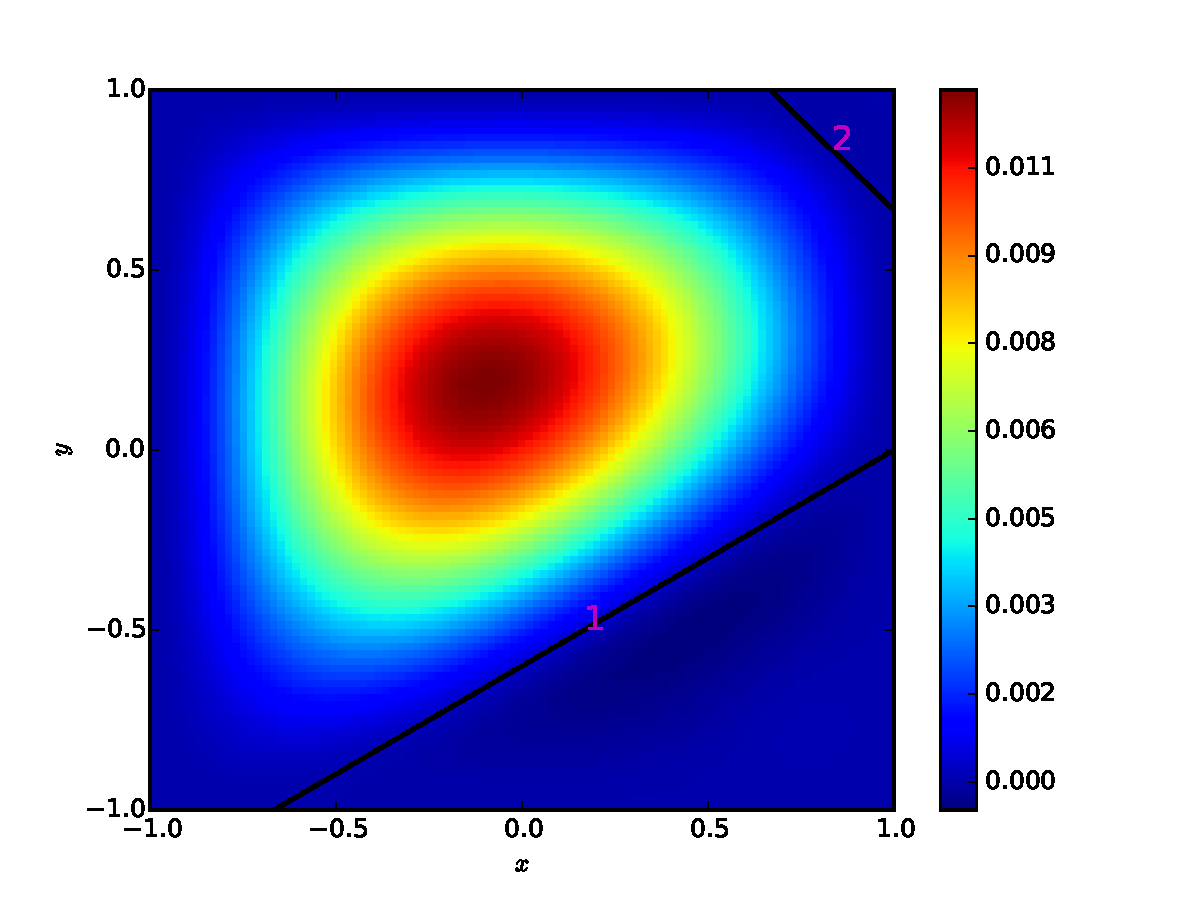
\includegraphics[width=0.45\textwidth]{img/shen_u0}
 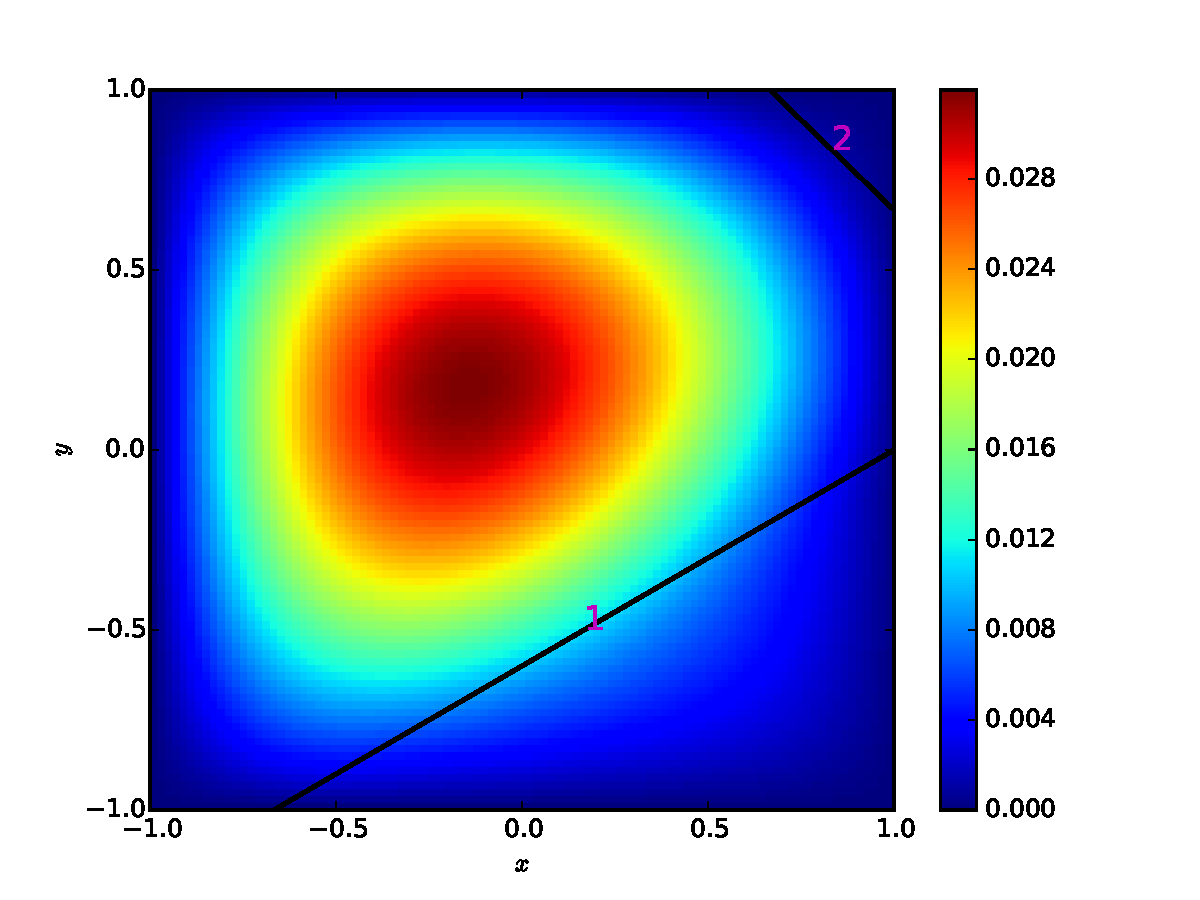
\includegraphics[width=0.45\textwidth]{img/sine_u0}\\
 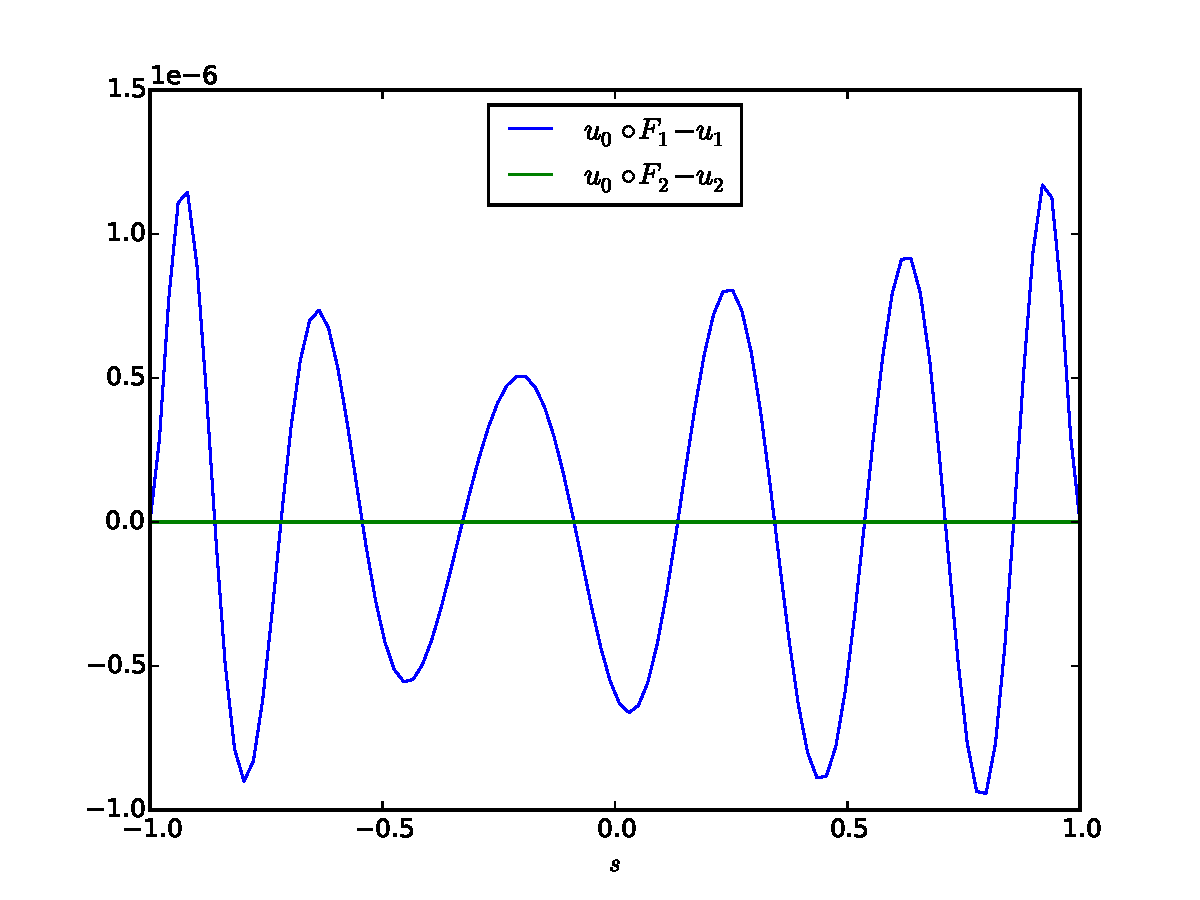
\includegraphics[width=0.45\textwidth]{img/shen_u0_ur}
 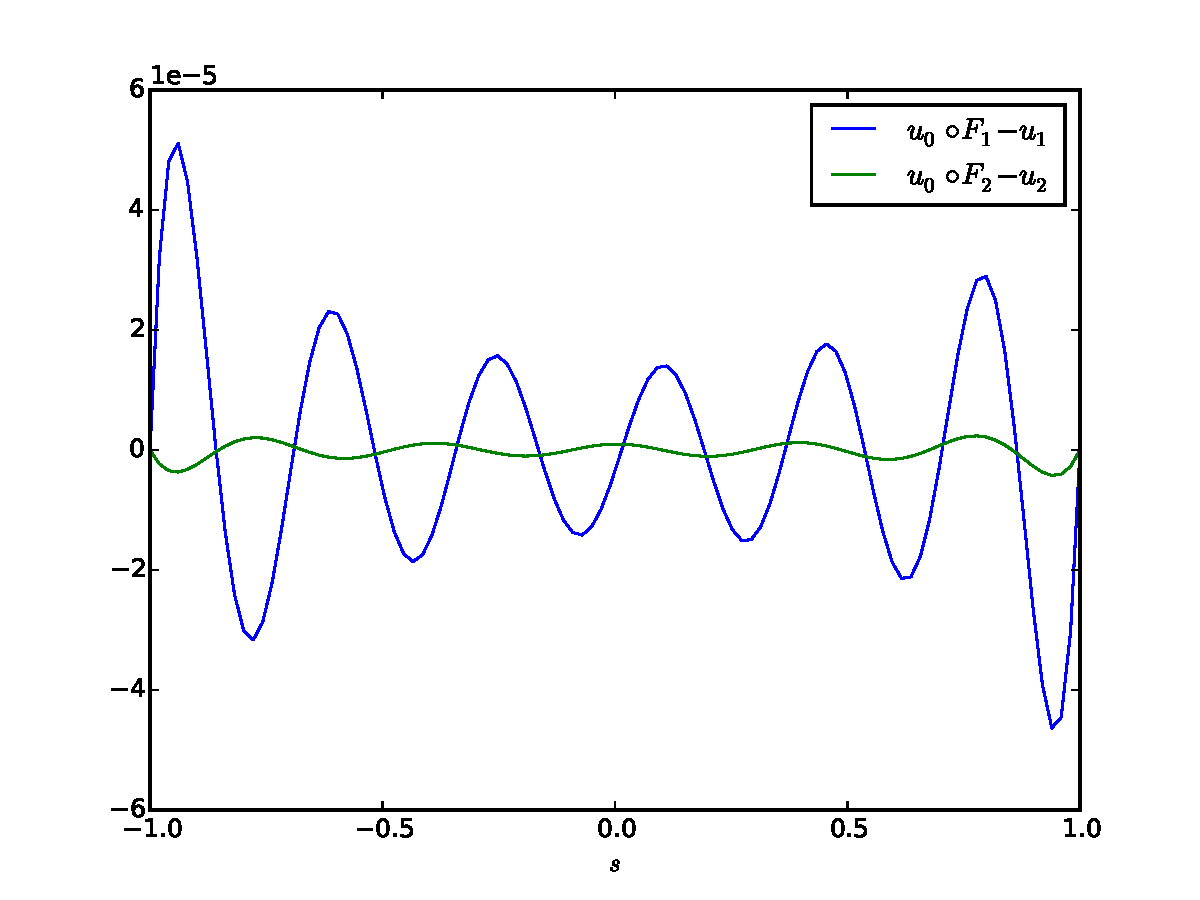
\includegraphics[width=0.45\textwidth]{img/sine_u0_ur}\\
 %\caption
 \caption{
  Solution of the plate-beam system obtained by the Galerkin method with Shen
  functions (left) and eigen functions (right) for $n=15$. In the top row the vertical
  displacement $u_0$ of the plate is plotted. The position of beams is indicated
  by black lines. Further the index of the beam is shown in magenta. In the
  bottom row the difference between the plate's displacement on the beams and the
  beams' displacement is shown. The error of constrains is less than $10^{-4}$.
 }
 \label{fig:solutions}
 \end{figure}

\section{Condition numbers of plate-beam systems and preconditioning}
\label{sec:lbb}
In this section we briefly discuss a phenomena which is bound to occur in any
discretization of plate-beam system, namely, the condition number of linear system 
grows with the size of the linear system (see e.g.
\cite{benzi}). This growth is due to the saddle point nature of the continuous
problem (\ref{eq:system}) but it can be greatly accelerated by the choice of the
discretization. To illustrate this issue let $\mathcal{A}_S$ be the symmetric
indefinite matrix in system (\ref{eq:sysAB}) obtained from discretization of
problem (\ref{eq:system}) by the Shen polynomials. Analogically, let
$\mathcal{A}_E$ be the matrix obtained by discretizing the problem with
eigenfunctions(odd trigonometric polynomials). Figure \ref{fig:no_precon} shows the 
spectral condition number $\kappa$ of both matrices $\mathcal{A}_S, \mathcal{A}_E$ 
as the function of the polynomials degree. The condition number of the matrix
$\mathcal{A}_S$ reaches the value of $\kappa=10^{15}$ very rapidly ($n=15$). For
the same degree the condition number of the eigenfunction system is about ten 
orders of magnitude smaller. We note that $n=15$ is a modest degree and to achieve
sufficient accuracy of the solution, spaces with larger dimensions might be
needed. However with larger spaces the linear systems quickly become stiff and
the obtained solution might suffer from round-off errors. This problem can be
avoided by solving a preconditioned problem. Here we shall hint on a part of the
suitable preconditioner. Note that for simplicity we set $E_r=1$ for all $r$.
 \begin{figure}[t!]
 \centering
 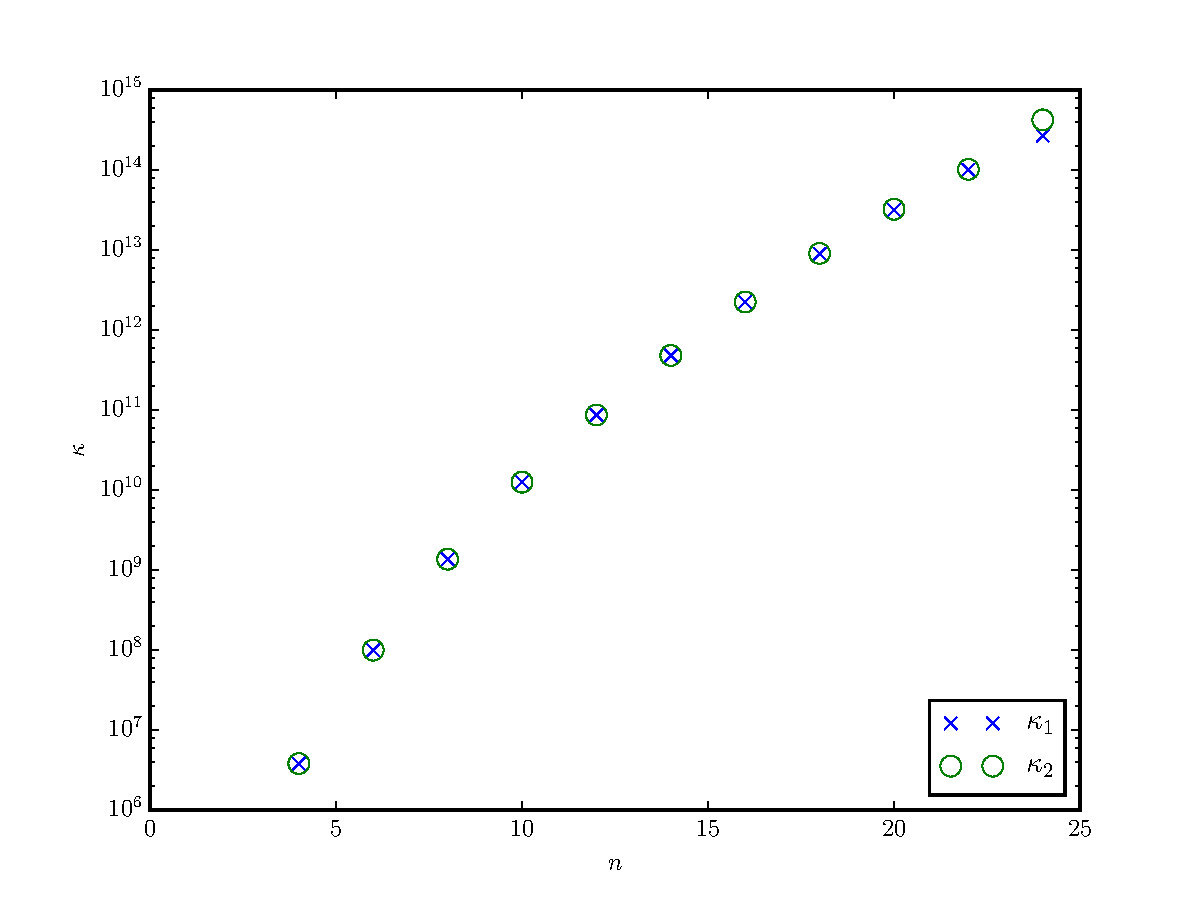
\includegraphics[width=0.45\textwidth]{img/shen_cond}
 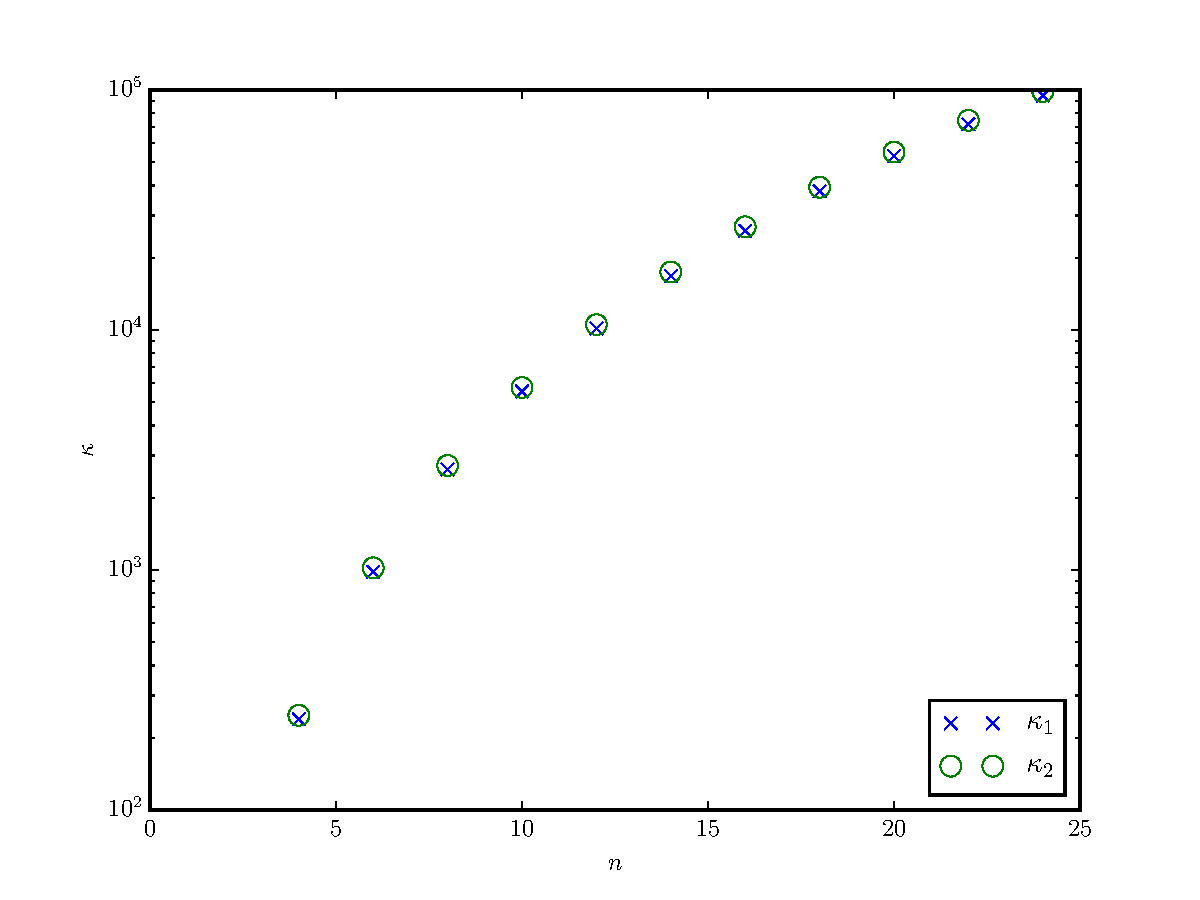
\includegraphics[width=0.45\textwidth]{img/sine_cond}\\
 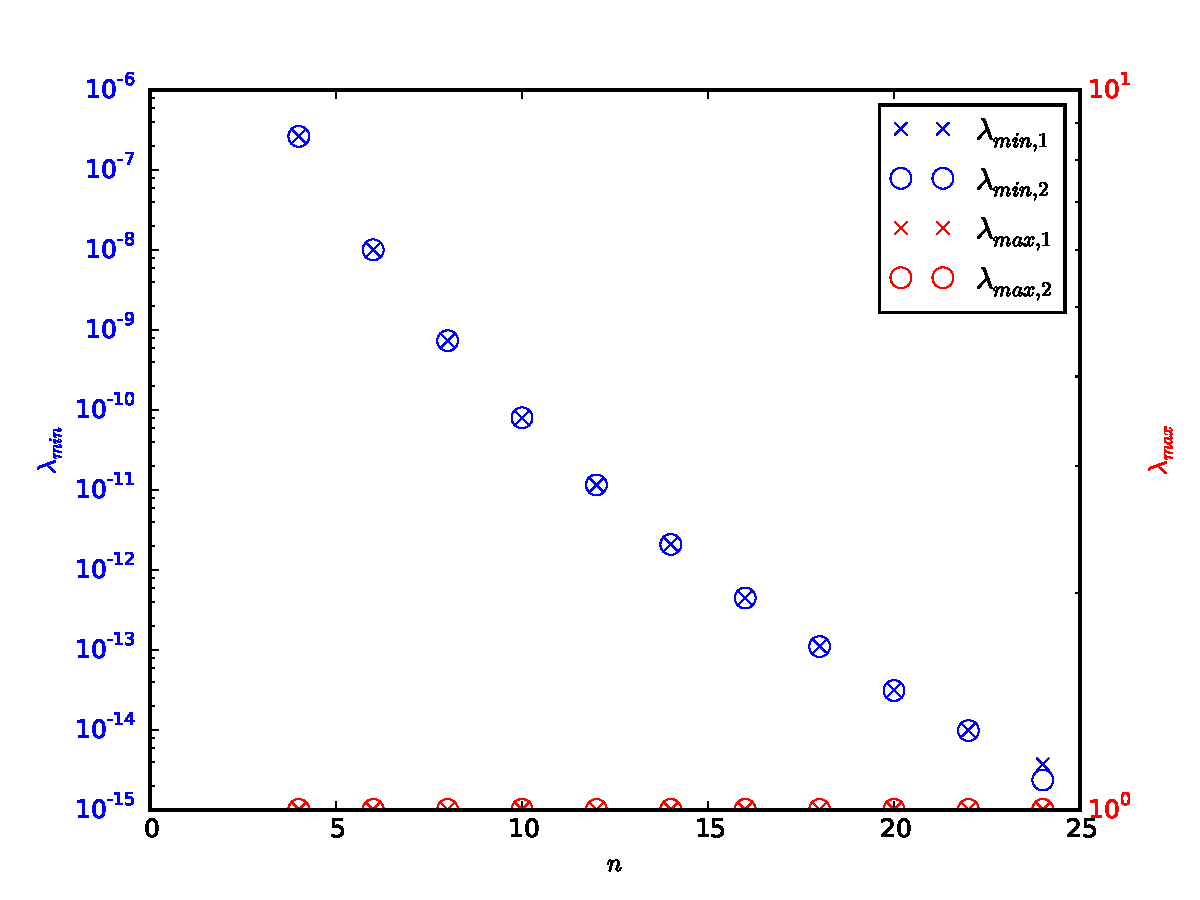
\includegraphics[width=0.45\textwidth]{img/shen_spectrum}
 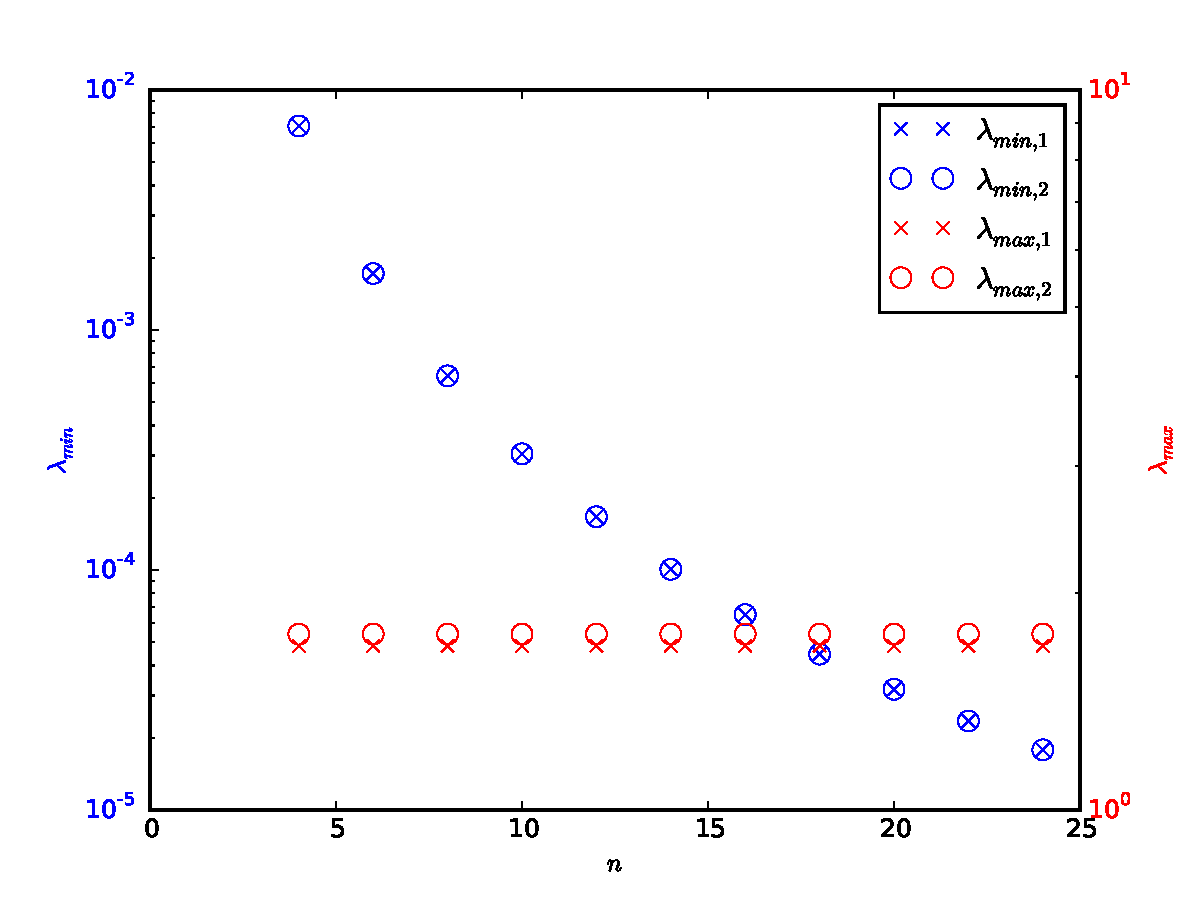
\includegraphics[width=0.45\textwidth]{img/sine_spectrum}\\
 \caption{Condition number $\kappa$ and spectra of linear systems $\mathcal{A}_S,
 \mathcal{A}_E$ stemming from discretization of the plate-beam system
 (\ref{eq:system})
 by Shen polynomials (left) and eigenfunctions (right) for different polynomial 
 degrees $n$. Two beam arrangements are considered. Subscripts one corresponds 
 to a single vertical beam $\left[0, -1\right]-\left[0, 1\right]$. Arrangement 
 where additional horizontal beam $\left[-1, 0\right]-\left[1, 0\right]$ is added 
 is denoted by subscript two. For both discretizations the condition numbers
 increases and the rate is significantly larger for the Shen basis. Presence 
 of the second beam has little to no effect on the rate. In the bottom row the 
 dependence of the smallest and largest eigenvalues $\lambda_{min}, \lambda_{max}$ 
 of matrixes $\mathcal{A}_S, \mathcal{A}_E$ on the degree $n$ is shown.
 The largest eigenvalues are stable, while the smallest ones approach zero and are
 thus the cause of the growth of the condition number $\kappa$. Consistent with
 the faster growth in the condition number of $\mathcal{A}_S$ its smallest
 eigenvalue decreases more rapidly than the smallest eigenvalue of
 $\mathcal{A}_E$. Note that both scales use logarithmic vertical axis.}
 \label{fig:no_precon}
 \end{figure}

Investigating the spectra of matrices $\mathcal{A}_S, \mathcal{A}_E$ in Figure 
\ref{fig:no_precon} it is clear that the growth of the condition number is mainly 
due to the fact that the smallest eigenvalue of the system decreases with the size of the linear
system/polynomial degree $n$. Using results of \cite{marie} that build on the work 
of \cite{malkus}, the smallest eigenvalue defines the discrete Brezzi inf-sup 
constant $\beta$, which determines stability of the discretization. In \cite{marie} 
stability of the finite element discretization of the Stokes(saddle point) system 
is investigated using the eigenvalue problem for the Schur complement
\begin{equation}
  \label{eq:schur}
  \Bmat^{\text{T}}\Amat^{-1}\Bmat\Pvec = \beta\mathbb{N}\Pvec,
\end{equation}
where $\mathbb{N}$ is a symmetric positive definite matrix which
represents discretization of the norm on the continuous space $Q$. The matrix is
\textit{a priori} known and the discretization is found stable if there exists a
universal lower bound on the smallest of eigenvalues $\beta$. That is, stable
discretization requires that the smallest eigenvalues $\beta$ are bounded from
below by a constant independent of the size of the linear system/polynomial
degree. Here we shall reverse the process: the matrix $\mathbb{N}$ is to be found 
from the requirement that the smallest eigenvalue remains bounded. It can be 
shown that such a matrix can be found by the following algorithm. Let $\mathbb{M},
\mathbb{A}$ the mass matrix and the matrix of the biharmonic operator on $\Qh$.
Then
$\mathbb{N}=\left(\mathbb{M}\mathbb{V}\right){\Lambda}^{-1}\left(\mathbb{M}\mathbb{V}\right)^{\text{T}}$,
where $\mathbb{V}$, $\Lambda$ solve the generalized eigenvalue problem
$\mathbb{A}\mathbb{V}=\mathbb{M}\mathbb{V}\Lambda$. Note that the negative power 
of the diagonal eigenvalue matrix $\Lambda$ suggests that the continuous spaces 
for the Lagrange multipliers will be Sobolev spaces with negative index.
Also note that with the basis of eigenfunctions we have $\mathbb{M}=\mathbb{V}=\mathbb{I}$
and $\Lambda=\mathbb{A}$. Thus there is no need to solve the generalized
eigenvalue problem. 

The smallest eigenvalue of the problem (\ref{eq:schur}) 
with the constructed matrix $\mathbb{N}$ is shown in Figure \ref{fig:schur}. 
The eigenvalue remains constant for all values of discretization parameter $n$.
 \begin{figure}[h!]
 \centering
 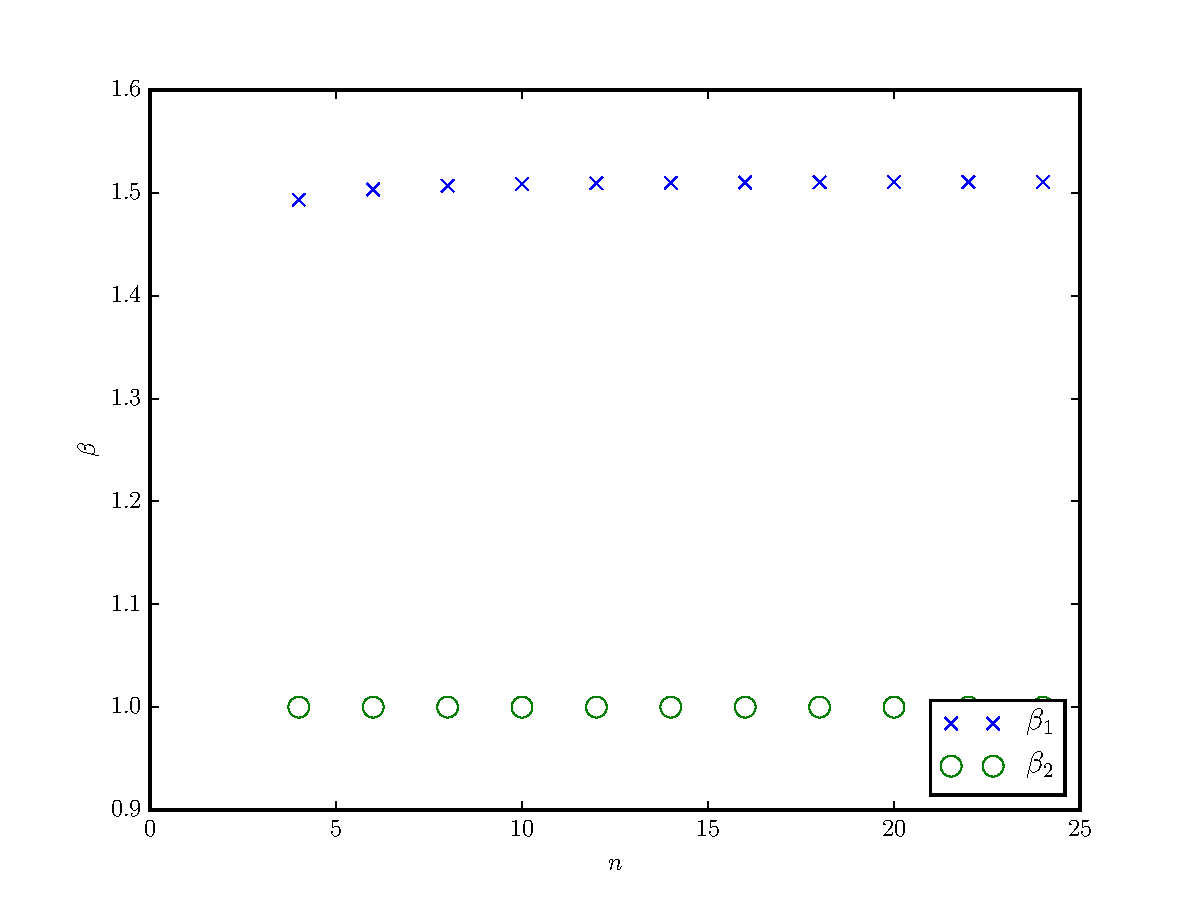
\includegraphics[width=0.45\textwidth]{img/Schur_precond_shen_cond}
 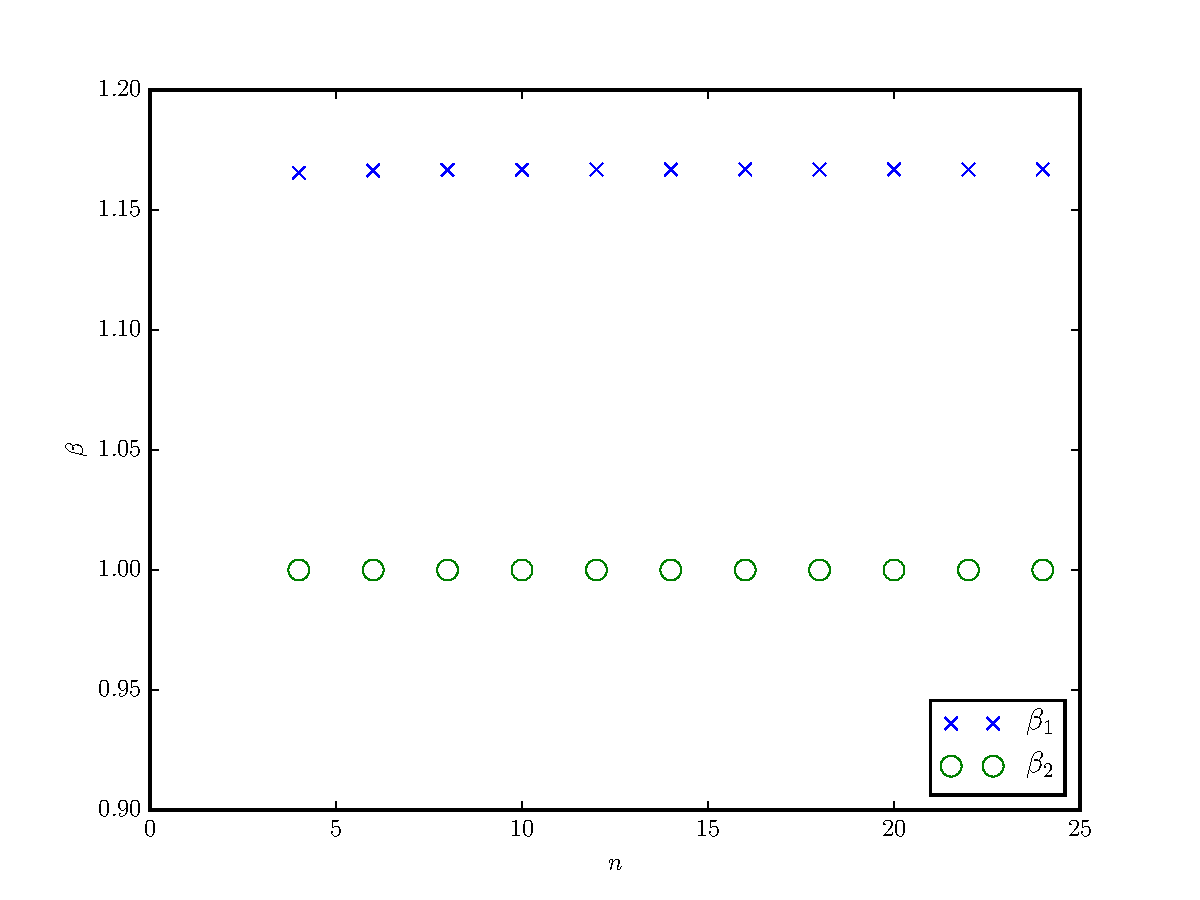
\includegraphics[width=0.45\textwidth]{img/Schur_precond_sine_cond}\\
 \caption{Smallest eigenvalues of the problem (\ref{eq:schur}) with constructed
 matrix $\mathbb{N}$. On the left the system was discretized with function due
 to Shen. Result of the system discretized with eigenfunctions are shown on the
 right. The smallest eigenvalue $\beta_1, \beta_2$ for the system with one and
 two beams remain constant for all polynomial degrees $n$.}
 \label{fig:schur}
 \end{figure}

Based on our findings and the theory of operator preconditioners reviewed in
\cite{kent} or the note of Murphy et al. \cite{golub} a possible preconditioner 
for the plate-beam (\ref{eq:sysAB}) system is a block diagonal matrix
\begin{equation}
\label{eq:prec}
\mathcal{P} = 
    \begin{bmatrix}
      \mathbb{A}^{-1} & 0 \\
      0 & \mathbb{N}^{-1}
    \end{bmatrix}.
\end{equation}
Here $\mathbb{A}, \mathbb{N}$ are generic matrices from the system
(\ref{eq:system}) and the suggested algorithm that approximates the Schur
complement (\ref{eq:schur}). We shall denote $\mathcal{P}_S, \mathcal{P}_E$ the 
preconditioners obtained from (\ref{eq:prec}) by substituting respectively the 
matrices obtained from discretizations by Shen polynomials and eigenfunctions.
Note that the preconditioner $\mathcal{P}_S$ is very cheap to compute. In fact it 
is a diagonal matrix with tabulated values.

The effect of the proposed preconditioner is shown in Figure \ref{fig:precond},
which shows the spectral condition number and the smallest and largest
eigenvalues of the preconditioned system $\mathcal{P}_S\mathcal{A}_S$ and 
$\mathcal{P}_E\mathcal{A}_E$. The preconditionesr have stabilized the smallest 
eigenvalues but at the same time linear growth has been introduced to the largest 
eigenvalues. The growth translates into a linear increase of the condition number 
of the systems. This is certainly an improvement over the case without the
preconditioner. However the ideal preconditioner would yield stable condition 
numbers. Moreover the preconditioner has to be robust with respect to the 
material/geometry properties $E_0, E_r, r\in R$ as well as the arrangement of
the beam. This aspect of the preconditioner (\ref{eq:prec}) has not been 
investigated here.
 \begin{figure}[t!]
 \centering
 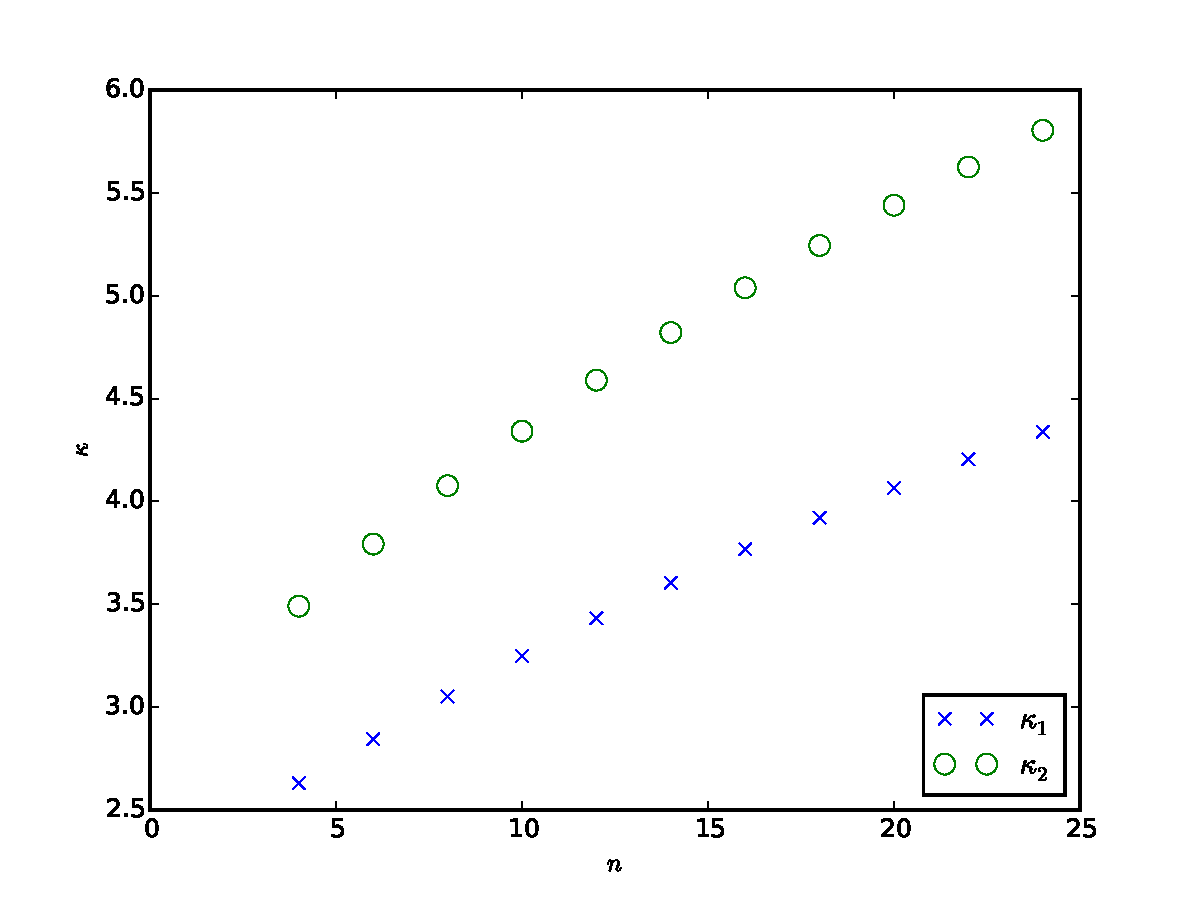
\includegraphics[width=0.45\textwidth]{img/Precond_shen_cond}
 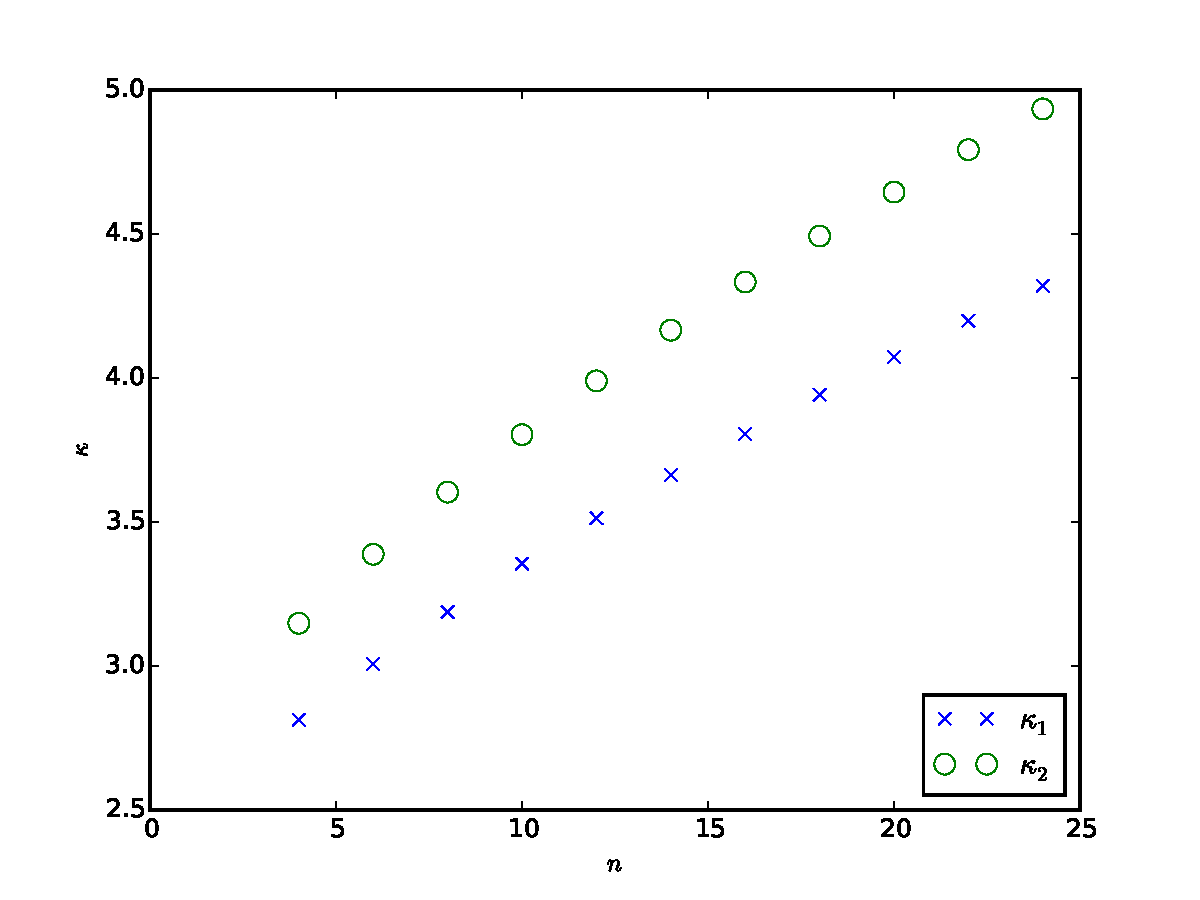
\includegraphics[width=0.45\textwidth]{img/Precond_sine_cond}\\
 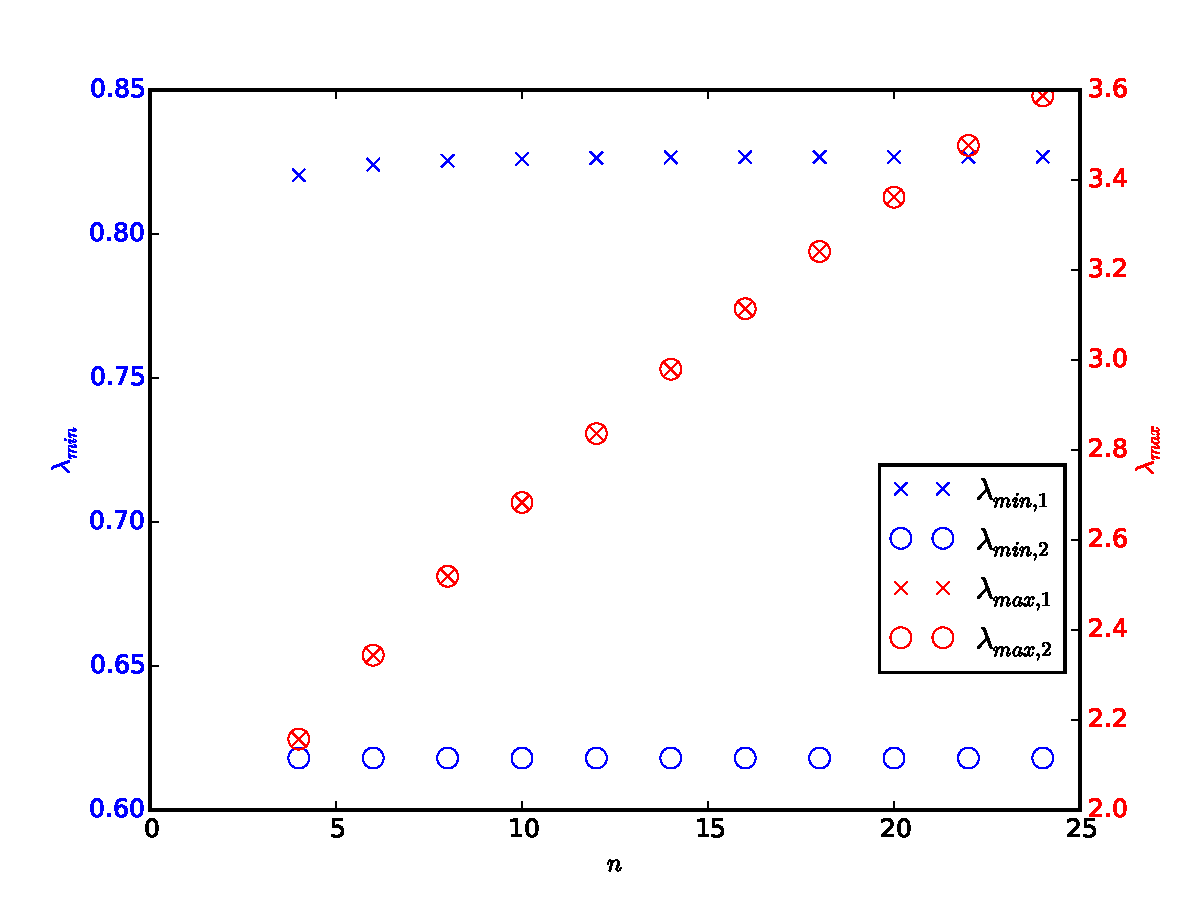
\includegraphics[width=0.45\textwidth]{img/prec_shen_spectrum}
 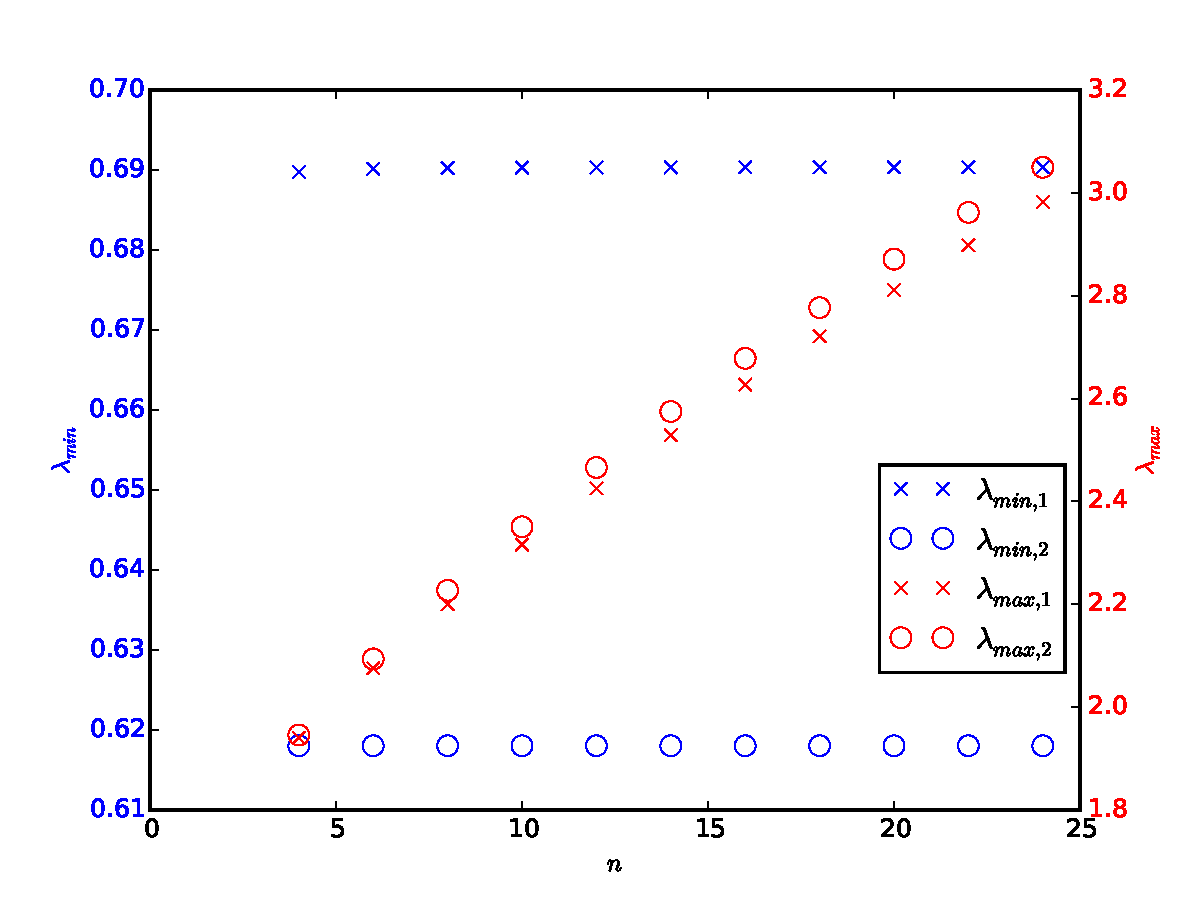
\includegraphics[width=0.45\textwidth]{img/prec_sine_spectrum}\\
 \caption{
 Condition number $\kappa$ and spectra of the preconditioned linear systems 
 $\mathcal{P}_S\mathcal{A}_S$ and $\mathcal{P}_E\mathcal{A}_E$
 stemming from discretization of the plate-beam system (\ref{eq:system}) and
 specializing (\ref{eq:prec}) by Shen polynomials (left) and eigenfunctions (right) 
 for different degrees $n$.
 Two beam arrangements are considered. Subscripts one corresponds to a single vertical beam
 $\left[0, -1\right]-\left[0, 1\right]$. Arrangement where a horizontal beam 
 $\left[-1, 0\right]-\left[1, 0\right]$ is added is denoted by subscript two.
 For both discretizations the condition numbers grows linearly with $n$. The growth 
 is due the growth of the largest eigenvalues of the systems. Presence of the
 second beam seems to have negligible effect on the condition number.
 }
 \label{fig:precond}
 \end{figure}

\section{Conclusions}
\label{sec:end}
In this paper we have discussed generic mathematical abstractions that lead to efficient
implementation of Galerkin methods for the constrained optimization problem
describing the coupled deformation of a thin plate supported by an arbitrary arrangement 
of support beams. Two specific sets of basis functions based on linear combinations of 
Legendre polynomials and eigenfunctions of the one-dimensional biharmonic
operator have been described. Both methods have been implemented in a python package 
$\text{Bend}\!\left|\text{P}\right|\!\text{y}$ which was used to explore efficient 
preconditioners for the resulting linear system. Some elements of the efficient
preconditioner have been identified. A complete robust preconditioner is currently
being pursued and is the topic of future work.

%\bibliography{bendpy.bib}
\newpage
\begin{thebibliography}{16}

\bibitem{argyris}
Argyris J.H., Fried I., and Scharpf D. W.,
\newblock
The TUBA family of plate elements for the matrix displacement method,
\newblock {\em Aeronautical Journal}, 72:701--709, 1968.

\bibitem{babuska}
Babu\v{s}ka I.,
\newblock The finite element method with Lagrangian multipliers,
\newblock {\em Numerische Mathematik}, 20(3):179--192, 1973.

\bibitem{benzi}
Benzi M., Golub G.H. and Liesen J.,
\newblock Numerical solution of saddle point problems,
\newblock {\em Acta Numerica}, 14(1):1--137, 2005.

\bibitem{brenner}
Brenner S.C. and Scott R.,
\newblock {\em The Mathematical Theory of Finite Element Methods},
\newblock Texts in Applied Mathematics, Springer, 2008.

\bibitem{brennerip}
Brenner S.C. and Sung L.-Y.,
\newblock $C^0$ interior penalty methods for fourth order elliptic boundary value
  problems on polygonal domains,
\newblock {\em Journal of Scientific Computing}, 22-23(1-3):83--118, 2005.

\bibitem{brezzi}
Brezzi F.,
\newblock On the existence, uniqueness and approximation of saddle-point
  problems arising from Lagrangian multipliers,
\newblock {\em ESAIM: Mathematical Modelling and Numerical Analysis -
  Modélisation Mathématique et Analyse Numérique}, 8(R2):129--151, 1974.

\bibitem{malkus}
Malkus D.S.,
\newblock Eigenproblems associated with the discrete LBB condition for
  incompressible finite elements,
\newblock {\em International Journal of Engineering Science},
  19(10):1299--1310, 1981.

\bibitem{kent}
Mardal K.-A. and Winther R.,
\newblock Preconditioning discretizations of systems of partial differential
  equations,
\newblock {\em Numerical Linear Algebra with Applications}, 18(1):1--40, 2011.

\bibitem{morley}
Morley L.S.D.,
\newblock The triangular equilibrium element in the solution of plate bending
  problems,
\newblock {\em Aero. Quart}, 19:149--169, 1968.

\bibitem{quarteroni}
Quarteroni A.,
\newblock {\em Numerical Models for Differential Problems}, volume~2,
\newblock Springer, 2009.

\bibitem{reddy}
Reddy B.D.,
\newblock {\em Introductory Functional Analysis: With Applications to Boundary
  Value Problems and Finite Elements},
\newblock Springer, 1998.

\bibitem{marie}
Rognes M.E.,
\newblock Automated testing of saddle point stability conditions,
\newblock In {\em Automated Solution of Differential Equations by the Finite
  Element Method}, Springer, 2012.

\bibitem{shenpaper}
Shen J.,
\newblock Efficient spectral-Galerkin method I: Direct solvers of second-and
  fourth-order equations using Legendre polynomials,
\newblock {\em SIAM J. Sci. Comput.}, 15(6):1489--1505, 1994.

\bibitem{sympy}
{SymPy Development Team},
\newblock {\em SymPy: Python Library for Symbolic Mathematics}, 2014.

\bibitem{numpy}
van~der Walt S., Colbert S.C. and Varoquaux G.,
\newblock The NumPy array: A structure for efficient numerical computation,
\newblock {\em Computing in Science \& Engineering}, 13(2):22--30, 2011.

\bibitem{golub}
Murphy M.F., Golub G.H. and Wathen A.J.,
\newblock A note on preconditioning for indefinite linear systems,
\newblock {\em SIAM J. Sci. Comput.}, 21(6):1969-1972, 1999.

\end{thebibliography}
\end{document}
